\documentclass{ezb}
\usepackage[]{todonotes}
\usepackage{amsmath}
\usepackage{gensymb}
\usepackage{wrapfig}
\usepackage{longtable}
\usepackage{amssymb}
\usepackage[colorlinks,        	% Links ohne Umrandungen in zu wählender Farbe
   linkcolor=black,   			% Farbe interner Verweise
   filecolor=black,   			% Farbe externer Verweise
   citecolor=black    			% Farbe von Zitaten
]{hyperref}
\usepackage{booktabs}

\renewcommand{\thesubsection}{\alph{subsection}}
\begin{document}

% \maketitle{Nummer}{Abgabedatum}{Tutor-Name}{Gruppennummer}
%           {Teilnehmer 1}{Teilnehmer 2}{Teilnehmer 3}
\maketitle{05.06.15}{Udo Frese}{1}{Annika Ofenloch - 2992807 - ofenloch@uni-bremen.de}{Frank Ihle - 3010158 - fihle@uni-bremen.de}{Simon Schirrmacher - 4000884 - simons@informatik.uni-bremen.de}{Noshaba Cheema - ncheema@uni-bremen.de}

%-------Text-Start------------------------------------------
\section{Ballspiele II}
\newpage
\section{Freistoß (4 Punkte)}
Bei einer Fußball-TV-Übertragung soll für den Zuschauer die Zone in das Bild eingezeichnet werden, auf der sich kein Gegenspieler bei einem Freistoß befinden darf.
\subsection{Allgemein}
Der Algorithmus orientiert sich an bekannten Objekten, deren Dimensionen im physikalischen Raum ihm bekannt sind. Die meißten Bemaßungen auf einem Fußballfeld sind festgeschrieben und falls es hiervon Abweichungen gibt, können diese vor Spielbeginn eingeholt und händisch eingetragen werden.\\
\linebreak
Das Fußballfeld ist rechteckig, aber je nach Blickwinkel der Kamera ergeben sich Bildverzerrungen (wenn beispielsweise, die Kamera flach, von der Seite und mittig auf das Spielfeld schaut, hat der Platz aus dieser Perspektive eine Trapezform). Von dieser Verzerrung muss auch der Kreis beeinflusst werden. So wird aus dem Kreis eine Ellipse, deren kurze Diagonale umso größer wird, je näher die Ellipse an der Kamera ist. Diese Verzerrung kann durch die Kameragleichung ermittelt werden (siehe Gleichung \ref{eq:Kameragleichung})\\
\linebreak
Wenn nun bekannt ist, mit welchen Parametern die Ellipse eingezeichnet werden soll, gibt es zwei Möglichkeiten hierfür. Zum einen kann man statisch festlegen, dass das Kamerabild genau an einer Stelle stehen bleibt und erst beim Anspielen wieder geschwenkt werden darf, da sich hier nun wieder der Kreis auflösen soll - so muss die Zone nur einmal berechnet und eingetragen werden, für die nachfolgenden Bilder kann diese dann einfach reinkopiert werden. \\
\linebreak
Die andere Möglichkeit ist, den Kreis beim Zoom-Vorgang zu zeigen. Hierfür werden min. zwei Bilder benötigt, auf denen Objekte zu sehen sind, deren reale Größe bekannt sind. Im Mittelpunkt der Bilder ist der Ball und es werden wie gewohnt die Ellipsen berechnet. Da beim Zoomen aber sich die Zone im Folgebild vergrößert, kann nun ein $\vartriangle r$ berechnet werden und für die nächsten Aufnahmen (und vor allem für diese, wo kein Objekt mit bekannter Größe zu erkennen ist) der Radius und dadurch die Ellipse definiert werden. Da dies einer linearen Zoom-Funktion entspricht, funktioniert dies in der Form nur bei konstanter Vergrößerungsgeschwindigkeit. Wenn mehr als zwei Aufnahmen zur Berechnung von $\vartriangle r$ verwendet und deren Ergebnis gemittelt werden, lässt sich dieser Faktor genauer einstellen.
\subsection{Skaliergrößen}
Nachfolgend, Beispiele für Objekte mit bekannten Ausmaßen, mit deren Hilfe letztlich die Freistoßzone definiert werden kann: Torlatte- und pfosten, Rasenmuster und die weiße Linien (darunter: Seiten- und Mittellinien, Strafraum und Anstoßkreis. 
\subsection{Kameraeinstellung}
Ein Bildpunkt im Weltkoordinatensystem kann auf das Kamerasystem mit nachfolgender Gleichung umgerechnet werden:\\
\begin{small}
\begin{equation}
\left(
\begin{array}{c}
      u \\
      v
\end{array}
\right)
=
\left(
\begin{array}{c}
      u_{0} \\
      v_{0}
\end{array}   
\right)
+ \alpha \cdot d_{\kappa1 ,\kappa2}(p(T^{-1}_{W\leftarrow C}\cdot p^{W})) 
\label{eq:Kameragleichung}
\end{equation}
\end{small}
Die Transformationsmatrix wird mit der nachfolgendne Gleichung \ref{eq:Transformationsmatrix} beschrieben.\\
\begin{small}
\begin{equation}
\textbf{T}_{W\leftarrow B}=
\begin{pmatrix}
1 & &  & x_{Ball} \\
 & 1 & & y_{Ball} \\
 & & 1 & z_{Ball} \\
 & & & 1
\end{pmatrix}
\cdot
\begin{pmatrix}
1 & &  & \\
 & cos \alpha_{r} & -sin \alpha_{r} & \\
 & sin \alpha_{r} & cos \alpha_{r} & \\
 & & & 1
\end{pmatrix}
\cdot
\begin{pmatrix}
cos \beta_{r} & & sin \beta_{r} & \\
 & 1 & & \\
-sin \beta_{r} & & cos \beta_{r} & \\
 & & & 1
\end{pmatrix}
\cdot
\begin{pmatrix}
cos \gamma_{r} & -sin \gamma_{r} & & \\
sin \gamma_{r} & cos \gamma_{r} & & \\
 & & 1 & \\
 & & & 1
\end{pmatrix}
\label{eq:Transformationsmatrix}
\end{equation}  
\end{small}
\linebreak
Hier sind $\alpha_{r}, \beta_{r}, \gamma_{r}$ die Winkel zwischen dem ursprünglichen und dem, um jeweils die drei Achsen verdrehtem, Koordinatenkreuz, die allerdings variabel sind. Repräsentativ für die anderen Winkel, soll die Winkelberechnung anhand der Beziehung für $\alpha_{r}$ erläutert werden, die in Abb. \ref{abb:alpharBerechnung} veranschaulicht wird.\\
\linebreak
Die blaue Strecke teilt das Feld in zwei Bereiche auf, sie ist gleichzeitig die Spiegelachse für $alpha_{r}$ und orientiert sich an der Kameraposition (hier ist x=0). So haben Strecken, die parallel zur Torlinie verlaufen, aus dieser Perspektive, in der linken Hälfte eine positive Steigung und in der rechten eine negative Steigung. Aus diesem Grund muss hier auch eine Fallunterscheidung gemacht werden. So wird $\alpha_{r}$ dann immer über das Winkel/Positionsverhältnis berechnet, wie in Gleichung \ref{eq:alphar} beschrieben. Eine Ähniche Berechnung muss dann für die beiden anderen Verdrehungswinkel des Koordinatenkreuzes durchgeführt werden ($ \beta , \gamma$) 
\todo[inline]{
-Per Schaubild verdeutlichen wieso man alle winkel braucht.\\
-dk1k2 ausformelieren ?
}.
\begin{equation}
\alpha_{r} = 
\begin{cases}
	\frac{\pi}{2} - (\frac{\pi}{2}-\alpha_{1,min}\frac{b'}{x}) & wenn \ x\geq 0  \\
    \frac{\pi}{2} - (\frac{\pi}{2}-\alpha_{2,min}\frac{b-b'}{x}) & wenn \ x\leq 0 \\
\end{cases}
\label{eq:alphar}
\end{equation}
\begin{figure}[!h]
\centering
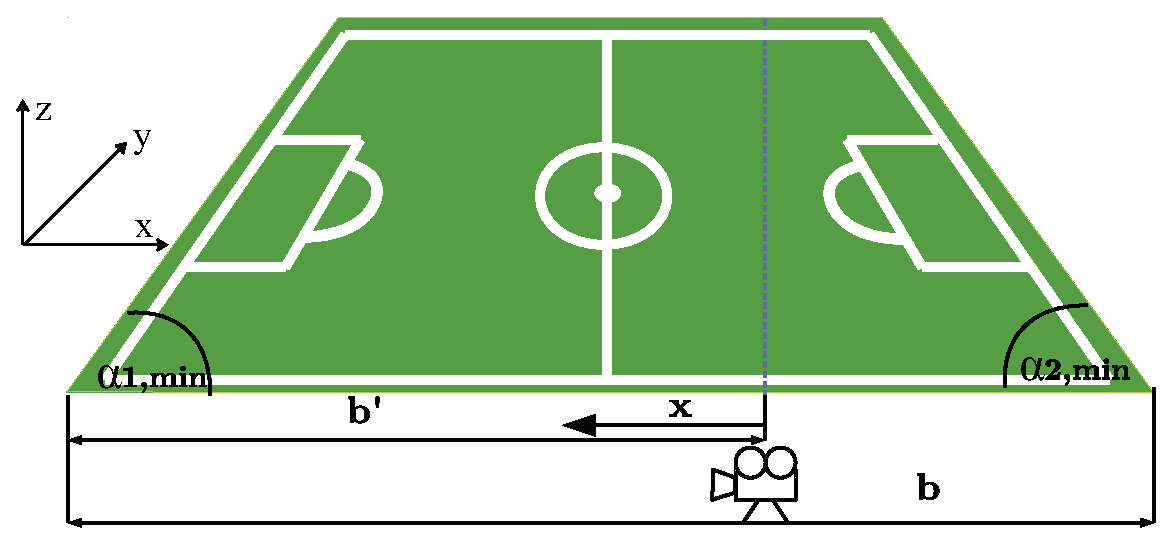
\includegraphics[scale=0.6]{./ar.eps}
\caption{Veranschaulichung für die $\alpha_{r}$-Berechnung}
\label{abb:alpharBerechnung}
\end{figure}
\subsection{Beurteilung}
Da beim Fußball schon wenige cm entscheidend sind, sollte der einzusetzende Algorithmus genaue Ergebnisse liefern, da \glqq Fehlentscheidungen\grqq \ ansonsten den Zuschauer verärgern können. Die unter diesen Bedingungen, gezeigten Methoden haben vermutlich nur eine begrenzte Genaugikeit, je nachdem wie exakt ein Objekt mit bekannter Größe erfasst wird (Negativbeispiel: Auflösung des Fußballs bei Aufnahme aus der Entfernung).
\section{Der einäugige Ballfangkönig (1 Punkt)}

%-------Text-End------------------------------------------
\end{document}

